\documentclass[10pt,a4paper,twocolumn]{article}
\usepackage[a4paper,margin=17mm,columnsep=6mm]{geometry}
\usepackage[T1]{fontenc}
\usepackage{newtxtext,newtxmath}
\usepackage{microtype}
\usepackage{amsmath}
\usepackage{booktabs}
\usepackage{graphicx}
\usepackage{xcolor}
\usepackage[font=small,labelfont=bf,skip=4pt]{caption}
\usepackage{enumitem}
\usepackage[hidelinks]{hyperref}
\usepackage{tabularx}
\usepackage{array}
\setlist{nosep,leftmargin=*}
\graphicspath{{fig/}{../../}}
\newcommand{\Npass}{212}
\newcommand{\Nmiss}{35}
\newcommand{\MissA}{10}
\newcommand{\MissB}{0}
\newcommand{\MissC}{15}
\newcommand{\MissD}{2}
\newcommand{\MissE}{7}
\newcommand{\MissF}{1}
\newcommand{\MissG}{0}

\renewcommand{\arraystretch}{1.08}
\setlength{\tabcolsep}{4pt}
\raggedbottom
\renewcommand{\topfraction}{0.92}\renewcommand{\dbltopfraction}{0.92}\renewcommand{\bottomfraction}{0.6}
\renewcommand{\textfraction}{0.06}\renewcommand{\floatpagefraction}{0.85}\renewcommand{\dblfloatpagefraction}{0.85}
\setcounter{topnumber}{3}\setcounter{dbltopnumber}{3}\setcounter{totalnumber}{5}
\makeatletter\setlength{\@fptop}{0pt}\setlength{\@dblfptop}{0pt}\makeatother
\begin{document}

\twocolumn[
\begin{@twocolumnfalse}
\begin{center}
{\LARGE\bfseries Flight Dynamics of the X-57 Maxwell in JSBSim\par}
\vspace{6pt}
{\large\bfseries A built-up model with fourteen propellers, proved on the Tecnam P2006T and checked against published CFD, tests and simulation\par}
\vspace{10pt}
{\large Technical report \quad\textbullet\quad November 2026\par}
\vspace{10pt}
\end{center}
\begin{abstract}
\noindent
A flight-dynamics model of the X-57 Maxwell in its Mod III and Mod IV forms has been written in JSBSim for the FlightGear simulator.
Mods III and IV never flew, so nothing here can be compared with a flight of those aircraft: the references are the CFD
database, wind tunnel and vibration tests of their parts, and piloted-simulation results, all published. The model is built up part by part, 17 wing strips a side, 3 stabilator strips a side, 4 fin strips and 11 fuselage stations, so that
any one of the fourteen propellers can fail and leave its own part of the wing. Each wing strip sits in the slipstream of its own disc, carried by the
ring-vortex wake used in the same author's helicopter models with one fitted constant, in place of the three a plain jet needed. The method was first proved on the
Tecnam P2006T, whose fuselage and tail the X-57 keeps: it passes that aircraft's flight manual, cruise within 2.7\,kt at 27 points and climb on one and two engines
within limits. Its flight-test misses are traced to the test paper's methods by a second source: at the Mod II simulator's mass the model gives
that simulator's short period within 5\,\%, and the paper's own derivatives give 4.95\,rad/s where its flight figure is 3.41. On the X-57 the model
reproduces the CFD's clean and flapped lift, the propellers' added lift inside the solvers' own spread, a cruise propeller's lift, drag reduction, pitch and roll on its wing within 21\,\% unfitted, and cruise $L/D$ of 14.2 against 13.5. Its modes follow the published
simulator's within 0.03 of damping and 10\,\% of frequency for Mod III. A motor lost with no pilot follows the published time histories: at 3\,s bank $-75^\circ$, pitch
$-10.1^\circ$, heading $-23.2^\circ$ against about $-87^\circ$, $-11^\circ$, $-23^\circ$, once the run is flown in the configuration the published traces show rather than the one their text
states. All limits were set before the results and none was moved, though one check's target was corrected (section~\ref{sec:review}): \Npass{} checks pass and \Nmiss{} miss. Every miss is listed with its cause or marked open. The largest are climb after a motor
failure with distributed thrust, 86 against 360\,ft/min, the climbs with both cruise motors running, 70 to 170\,ft/min above the simulator's, and three frequencies against the Mod II simulator.
\end{abstract}
\vspace{6pt}
\end{@twocolumnfalse}
]

\section{Introduction}
The X-57 Maxwell was a battery-electric demonstrator built on a Tecnam P2006T \cite{tm}. Mod II replaced the two piston engines with electric motors in the same
places. Mod III replaced the wing with one of 42\,\% of the area, aspect ratio 15, and moved the cruise motors to the wingtips, where their propellers turn against the tip vortices. Mod IV
powers twelve folding high-lift propellers along the leading edge, which Mod III carries folded and inactive \cite{tm}, to bring the stall speed back to the P2006T's \cite{hlp}. The project ended with Mod II built and tested on the ground, the Mod III wing built and
vibration tested \cite{gvt}, and neither of the later forms flown.

That leaves an unusual problem for a flight model: a large and open body of data, with no flight to hold it to. The CFD database \cite{tm} covers the wing, flaps and propellers; the high-lift
propeller was tested in a wind tunnel \cite{tun}; the batteries, motors, controllers and cockpit are documented \cite{icd,pc,tr}; and the piloted simulator's results are published \cite{sim3,sim2,cm,dt}.
All of those except the tests are predictions. Holding one prediction to another shows only agreement, so each check here is labelled by what it is held to: \textbf{M} measured, \textbf{C} CFD,
\textbf{S} a published simulator, \textbf{D} a design document.

A table model on the database's own structure reproduces the CFD by construction, and is kept as the reference. It can't lose one motor's slipstream from one part of the wing except through the database's
increments. The model that ships is built up instead: strips, discs, tail and bodies, whose failures come out of the parts.

\begin{figure*}[t]
\centering
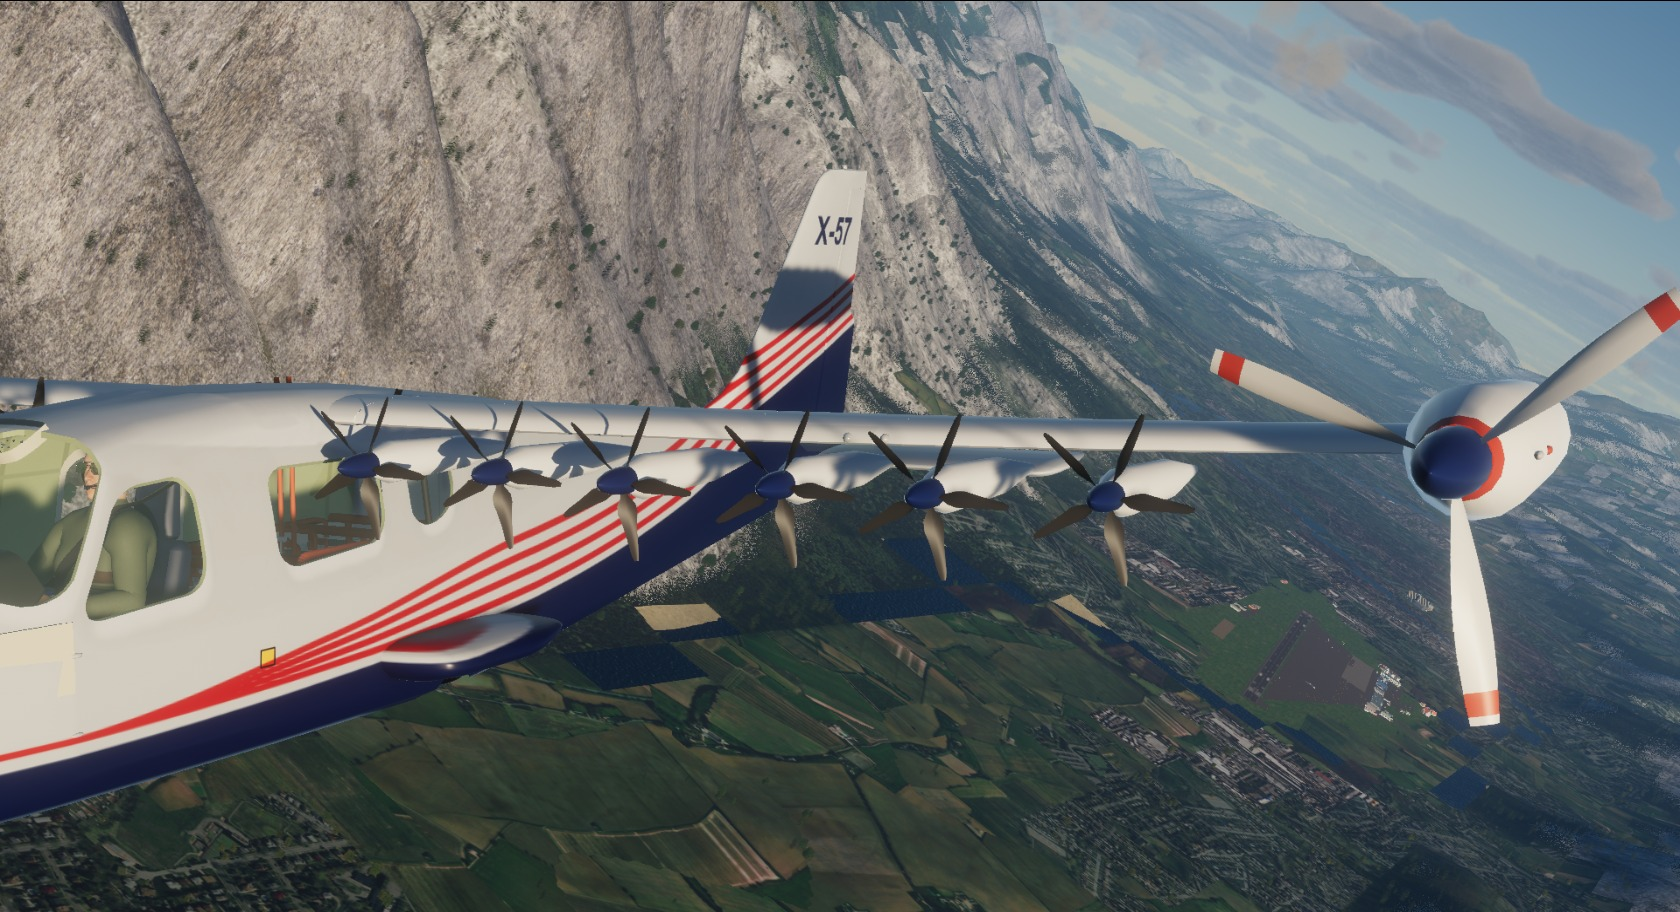
\includegraphics[width=0.74\textwidth]{X57.jpg}
\caption{The model in FlightGear: Mod IV in a banked turn with the high-lift propellers running.}\label{fig:x57}
\end{figure*}

\section{Reference data}\label{sec:ref}
When sources disagree the shipped model follows the highest-ranked: flight test of that aircraft with a clean method, then wind tunnel at a comparable Reynolds number and configuration,
then CFD, then a published simulator, then handbook estimates. A simulator ranks low because it's built from the others. The model is never tuned towards two sources at once. A
comparison with a simulator is run on that simulator's inputs (its mass, its trim, its configuration), so that what's left is the model's own error; a part that vanishes was only a difference
in data. Rank doesn't excuse a source from a sanity check: section~\ref{sec:p2006t} sets aside a higher-ranked figure for a stated reason.

\begin{table}[t]
\centering\small
\caption{Sources and what they contribute.}\label{tab:sources}
\begin{tabularx}{\columnwidth}{@{}>{\raggedright\arraybackslash}p{2.3cm}X@{}}
\toprule
Source & Content used \\
\midrule
TM-20250001715~\cite{tm} & CFD database, power off and on, ground planes, contactor failures, model structure \\
NASA OpenVSP model & geometry of wing, nacelles, blades \\
20210016834, 20220006506~\cite{tun,tun2} & high-lift propeller in the tunnel, blade weights \\
20240006496, 20230004174~\cite{sim3,sim2} & simulators: mass, modes, failures, Mod II's identification \\
20240006682, 20240010539~\cite{cm,dt} & motor failure histories, DiTTo climbs \\
20240011864, 20240007439~\cite{gvt,fl} & Mod III wing vibration test, flutter model \\
ICD-CEPT-006~\cite{icd} & cockpit, switches, sequences, displays \\
20240009560, 20240005892, 20170005797~\cite{tr,pc,pc17} & motors, controllers, power system \\
Chin et al.~\cite{chin} & cell model, thermal \\
P2006T flight manual~\cite{afm} & performance, stall, gear system \\
Nicolosi et al.~\cite{nic} & P2006T flight tests, tunnel, derivatives \\
\bottomrule
\end{tabularx}
\end{table}

\section{The model}\label{sec:model}
\subsection{Implementation}
One generator writes the Mod III, Mod IV and P2006T builds as plain JSBSim XML, with no scripting in the flight model. Forces and moments go through the aerodynamics axes. The build runs at 120\,Hz, a
rate at which the bending modes, flights and failures have converged. Inside FlightGear the force graph has to run as a system channel with stored outputs: read through FlightGear's property tree it would be
worked out again at each read, and the start never finishes. Every property read in FlightGear takes a lock, so the shipped graph is laid out to read few: functions read once are written into their reader, unread ones are dropped, and the high-lift channels rest while those propellers are stopped and disarmed. That takes Mod IV from about 6900 reads a step to 6600, or 5600 at rest. A check flies this build beside the plain one, and the two match to the last bit.

\subsection{Airframe}
\begin{figure*}[t]
\centering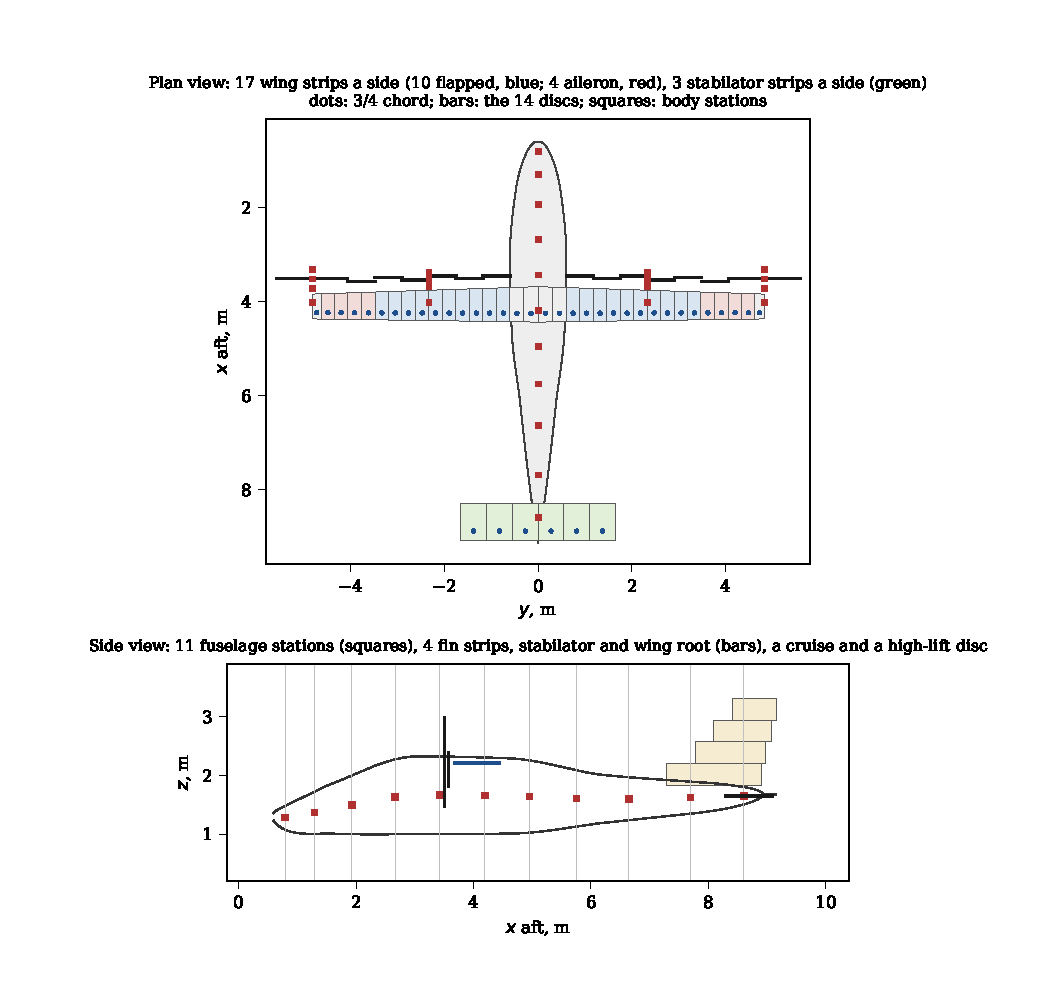
\includegraphics[width=\textwidth]{geometry.pdf}
\caption{The model's discretisation, drawn from the generator's data, Mod IV. Strips end at each disc's edge, and at the flap's and aileron's. The P2006T's build has 13 wing strips a side (6 flapped, 3 aileron, 2 on the winglet), with the same 3 stabilator and 4 fin strips and 11 fuselage stations. The tip nacelles have 4 stations each; the high-lift nacelles are lumped, six to a side at their mean span, also on 4 stations.}\label{fig:geometry}
\end{figure*}
The wing is 17 strips a side (fig.~\ref{fig:geometry}): 10 flapped, 4 with the aileron and 3 plain. Strips end at each propeller's edge, so that a disc's slipstream has strips of its own. Their sections from NeuralFoil on the geometry's own airfoils and a lifting-line solution for the spanwise loading. The fuselage's crossflow, a circle's doublet, reaches the strips beside it, which gives the high wing its dihedral effect; the strip over the cabin, inside that circle, carries the fuselage's carry-through lift as wing, so the loading runs on across without root vortices. The slotted flap's section lift, moment and drag are fitted to
the CFD at flaps 0, 10 and 30, power off, and flaps 20 is left out of the fit as a test. Tail, fin and bodies follow the method proved on the P2006T. Past 8$^\circ$ a pitching moment on body incidence carries what the strips can't, because the CFD's
pitch break comes at the same incidence with the propellers on or off, where a blown section is still short of stall. Rate derivatives are carried from the strips' to the tunnel-based ones the simulator uses,
because without that the roll modes run 19 to 34\,\% quick. With the high lift on, that correction holds its value from 2$^\circ$ under the power-off stall: past it, it stands for unblown sections stalling, which blown ones don't.

\subsection{Propellers and motors}
Propellers are discs, not blades: the blades of twelve propellers pass at 400\,Hz, far beyond the frame. Each of the fourteen discs keeps its own speed and takes the air at its own place, the airplane's roll, pitch and yaw included: a yaw rate speeds one wingtip's disc and slows the other's. Thrust, torque and in-plane force come from offline blade-element tables on the
published blades. The high-lift blades run about 10$^\circ$ folded forward on their hinges, so the tables use an effective 20.0$^\circ$ against 27.35$^\circ$ drawn: partly documented, partly fitted to the published schedule. The cruise propeller's speed is governed by its blade pitch, which an electric hub changes at 1$^\circ$/s, and each motor is a torque balance on the rotor's inertia. No rotor inertia is published. The cruise rotor's 0.65\,kg\,m$^2$ is about 0.5 for the propeller, from the manufacturer's 1997 data sheet (0.6\,kg\,m$^2$ with
160\,cm blades, scaled to 152\,cm), and 0.15 for the motor's rotor, estimated; the range is 0.58 to 0.73. The high-lift rotor's 0.0085 comes from the measured blade weights and the reference motor's parts \cite{hlm}.

The cruise propellers turn against the tip vortices, inboard blade rising: the published statements \cite{borer,dv} and the published 3-D geometry, measured blade by blade, agree. Each wing's six high-lift propellers turn the same way as its cruise propeller, the wings mirrored. The published geometry builds them so. The Mod IV CFD's skin friction \cite{dv} has the same lopsided pattern in every bay of a wing and its mirror image on the other, where alternating propellers would flip it from bay to bay. And on the X-57's predecessor wing, CFD gave propellers all turning against the tip vortex 0.31 more lift coefficient than pairs turning towards each other \cite{deere}. The simulator paper's ``each pair of motors was counter-rotating'' \cite{sim3} is taken as left against right. It can also be read as neighbours, as this model first did, so that simulator may differ.

\subsection{Slipstream}\label{sec:wake}
The axial speed at each strip comes from a tube of ring vortices behind the disc, after Heyson and Katzoff \cite{hk}, the model used for the same author's V-22, UH-60 and Bo 105. Its contraction, 0.90 of the radius, is momentum theory's. The
slipstream's effect on a wing is then reduced by one fitted constant, on the jet's strength:
\begin{equation}
a_\text{eff} = a\left(1 - k\,\frac{a}{u+a}\right),\qquad k = 0.70
\end{equation}
It probably stands for a jet no taller than the chord, which does less than strip theory says; that isn't proved. The plain momentum jet this replaced needed three fitted constants for much the same result (section~\ref{sec:hl}). In a sideslip each jet drifts with the crossflow, the less the stronger it is: per foot behind the disc, $-v/(u+1.5a)$ over the wing and $-v/(u+2a)$ at the tail, much as the same author's UH-60 carries its main rotor's wake to the tail by speed and direction. Each strip's share of each jet is a table on that drift, nil at none, so straight flight is as before. At 10$^\circ$ of sideslip it gives the CFD's growth of power-on roll as speed falls: $-0.035$ against $-0.048$ at 50\,KCAS, from $-0.024$. At 20$^\circ$ the CFD's roll grows faster than any drift gives. No dynamic inflow is
modelled: a Peters--He wake on each disc would give its own inflow, which the tables already hold in steady flow, and wouldn't change how the slipstream reaches the wing.

Each jet also turns, its swirl carrying the propeller's torque as angular momentum. The cruise propellers' loading is published: NASA's CFD gives them Goldstein's \cite{tm}, so their swirl follows the optimum's profile \cite{gold}, a solid body's inside $r/R = J/\pi$, a free vortex's outside it and nil at the tip (Prandtl's loss for three blades standing for Goldstein's), from the nacelle's surface out, scaled to the torque and spun up as the jet contracts. That puts 1.7 to 2 times an even swirl on the strip beside the nacelle, across $J$ 0.6 to 1.6; the model takes $J=1$. The swirl also turns the flow each strip's force stands on, so a strip in its upwash leans its lift forward: the slipstream's rotation won back as thrust, the reason the cruise propellers turn against the tip vortex. Behind the high-lift discs the swirl stays even from 0.35 of the radius out, a stand-in for an unpublished BEM loading, and leaves the force's direction alone: with wing on both sides of a hub the net lean is the difference of two large ones, and given the even swirl the high-lift drag fell further under the CFD's, 0.082 against 0.119 at flaps 10 from 0.106.
With one cruise propeller at the CFD's thrust, as the CFD runs it, 41 cases from 43 to 142\,KCAS, the model gives 1.07 of the CFD's added lift, 1.01 of its drag reduction and 0.88 of its pitch, rms errors 15, 48 and 21\,\% (the drag's 0.0012); the strips' own roll is 1.03 of the CFD's. With the swirl even and the force not turned it gave 0.73, $-0.99$, 0.39 and 0.71: drag rose with thrust where the CFD's falls. At 150\,KTAS the two now take 0.0023 off the cruise drag coefficient, where NASA's report puts the tip propellers' benefit at 0.0028 \cite{tm}. Nothing in this was fitted. The side force, nil in the model, and the yaw are under the 0.005 floor of the limit, as is the drag.

\subsection{Named fits}
Fits are named, and a fitted figure can't pass a check by itself. Besides the sections and those above: the flap's turning of the jet; the slipstream at the tail; a jet's lift from nearer the centre after a contactor failure; sideslip's roll and yaw on
sideslip, incidence and flap, from the CFD, power off, because the strips lose the windward lift near stall where the CFD keeps it, with the high lift on only its part at 2$^\circ$, far from stall; one propeller's roll from the published tables, less the strips' own share, because a windmilling propeller takes lift off its own wing, which the strips, fed by thrust, don't (powered, the strips now give the tables' roll on their own); the
rudder, whose section table ran out towards full travel; ground effect on height, incidence and flap, power off and on; the gear's drag area of 4\,ft$^2$, from the simulator's phugoid; and the brakes' force, from the P2006T's landing roll.

\subsection{Power, battery and cockpit}
The traction battery follows a cell model \cite{chin}. Seven avionics buses, the essential battery, two converters and their cross buses run inside the flight model, so that a shed bus or a failed converter
reaches the contactors and the motors as the handbook says \cite{icd}. Voltages are fixed and loads estimated. The cockpit's logic is in the aircraft's own files; the companion manual describes it.

\subsection{Wing bending and gear}
The wing bends in its first mode, symmetric and antisymmetric, as in the same author's ASK 21: stiffness fitted to the Mod III wing's vibration test \cite{gvt}, with tip masses and without, each nacelle a mass with the rotary inertia of its size. The panels' coupling to the airframe is solved in the system, with an effective
mass for each kind of motion. Tyre deformation drag follows the published equation \cite{gd}, held at its value past 55\,KIAS, where its fit ends. The brakes are the P2006T's, which the X-57 kept: a disc gives a torque for its pressure, so the pedal sets a force at each main tyre, capped by the tyre's grip. Their force at full pedal, 237\,lbf a wheel or about 0.2\,g with both, is fitted to the manual's landing roll. Gear terms reach the panels as the mean of two frames, which removes a 60\,Hz shake
between JSBSim's tyre friction and the panels' reaction.

\subsection{Mass}
FlightGear flies the published gross weights: 3000\,lb for Mod III \cite{tm} and a projected 3200\,lb for Mod IV \cite{fl}. Comparisons with the simulator run at its 3075\,lb. The 28.6\,\% CG and the inertias are the simulator's \cite{sim3}: no other is published.
With no fuel, weight and CG stay constant through a flight.

\section{Method}\label{sec:method}
The work went in phases, each with limits written before its first result, taken from the sources' own spread where they have one. A limit isn't moved afterwards, and a miss stays printed until its cause is fixed. One script refits the model and runs every check, at four processes.
Where a test's configuration turned out to be wrong it was changed and the old run kept printing beside it, with the reason given. Table~\ref{tab:checks} gives the count by group.

\begin{table}[t]
\centering\small
\caption{All checks, by what they're held to: M measured, C CFD, S a simulator, D a design document.}\label{tab:checks}
\begin{tabular}{@{}p{50mm}lrr@{}}
\toprule
Checks & Against & Pass & Miss\\
\midrule
Modes and CFD increments, built-up model (limits written for the table model) & C, S & 2 & 10\\
Propellers, motors, governor, battery & M, S & 24 & 0\\
P2006T: flight manual, flight tests, tunnel, Mod II simulator & M, S & 47 & 17\\
X-57 built-up aerodynamics against CFD & C & 37 & 1\\
Ground effect, climbs, failures, gear & C, S, M & 41 & 9\\
Wing bending & M, S & 31 & 1\\
Cockpit power and propeller modes & D & 27 & 0\\
\midrule
All & & 209 & 38\\
\bottomrule
\end{tabular}

\end{table}

\section{Results}\label{sec:results}
\subsection{The method on the P2006T}\label{sec:p2006t}
\textbf{(M)} The built-up method passes the P2006T's flight manual: 27 cruise points mean $+1.3$\,kt, rms 1.7, worst 2.7 (fig.~\ref{fig:cruise}, one drag fit); climb within limits on two engines and one, 1129 against 1102\,ft/min at maximum weight and 217 against 206 on one engine. Stall speeds are fitted. Against the tunnel, part by part, it gives
lift slope 0.0825/deg (0.080) and the neutral point 41.4\,\% (41). In flight, phugoid 28.8\,s (27), damping 0.088 (0.09); Dutch roll 2.96\,s (3.25), damping 0.305 (0.26).

Six checks against the flight paper \cite{nic} miss, and a second source says why. The simulator for Mod II was built on an identification of an instrumented P2006T and shown matching that aircraft's flight data \cite{sim2}, and its paper prints mass, CG and inertias, so the model can be run
at them \textbf{(S)}. Its short period then agrees across the range (fig.~\ref{fig:modii}): 3.85, 4.47, 5.13\,rad/s against 3.7, 4.4, 5.2, damping 0.53 to 0.56 against 0.59. The flight paper's 3.41\,rad/s and 0.40 are the outliers. Its maximum-slope method needs a true step, and the pilot's took about 0.6\,s: the same method on the model's response to a 0.6\,s step gives 3.68\,rad/s,
though the model's root is 5.92 at that mass and CG. The lift slope misses too, but the paper's 4.15/rad is the outlier again. Read together, because they share their points, the simulator paper's figures 11 and 12 give $C_L$ against $\alpha$: 5.09/rad, straight through all five cruise points. The nose vane appears to read about 1.3 of true incidence, and the simulator's authors replaced the
published slope themselves \cite{sim2}. The model's trimmed 5.70 is still 12\,\% above the simulator's, a real excess, and a miss. Aileron per degree of sideslip is 0.75 against the flight paper's 0.58 and, at the simulator's mass, 0.93 against its 0.80. The tunnel's $C_{Y\beta}$ of $-0.69$ stays open: sources run from $-0.36$ to $-0.69$, and the model gives $-0.48$, or $-0.65$ with winglets and power.

\begin{figure}[t]
\centering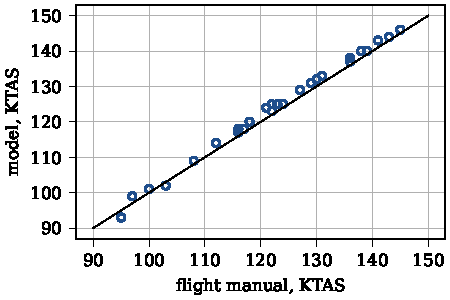
\includegraphics[width=0.78\columnwidth]{cruise.pdf}
\caption{P2006T cruise speed at the manual's power, 27 points \textbf{(M)}.}\label{fig:cruise}
\end{figure}

\begin{figure}[t]
\centering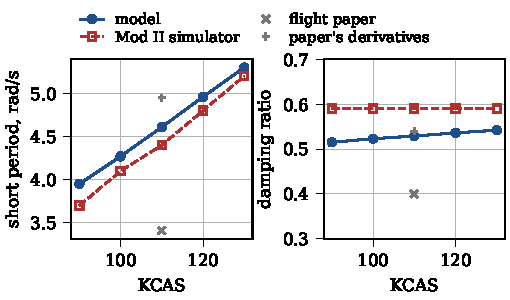
\includegraphics[width=\columnwidth]{modii.pdf}
\caption{Short period at the Mod II simulator's mass against that simulator, read by eye \textbf{(S)}. The flight paper's measured figure and the one its own derivatives give, at 110\,KIAS and its lighter mass and forward CG, are shown for scale.}\label{fig:modii}
\end{figure}

Against the same simulator three other frequencies miss. Dutch roll is 42\,\% high at 110\,KCAS (1.80 against 1.27\,rad/s), but scaling the flight test's 2.0\,rad/s by the inertia gives 1.75, so measurement sides with the model. Phugoid is 17 to 24\,\% high, and the flight test's 27\,s sides with the model again. The roll time constant is 0.1\,s against the simulator's 0.7 to 0.9\,s: any published $C_{lp}$ at the
printed inertia gives 0.1 to 0.2\,s, and the flight paper calls the mode too short to observe. That gap is unexplained.

None of this reaches the X-57's lift or stability, which come from the CFD: the P2006T is where the method was proved.

\subsection{X-57 aerodynamics}
\textbf{(C)} Power off, the fitted flaps match the solvers' mean within 0.003 in $C_L$ and 0.020 in $C_m$; flaps 20, unfitted, within 0.055 and 0.026. Unfitted increments below stall: stabilator $C_L$ 16\,\% and $C_m$ 7\,\% rms, aileron roll 16\,\%, sideslip side force 8\,\%. Sideslip's moments and the rudder are fitted now and are no longer tests, power off. With the propellers on they still are: 23 and 8\,\% rms of the increments in roll and yaw (limit 25). Trimmed stall speeds for Mod III are 82.7, 80.6 and 70.8\,KCAS against the published 88, 80, 73, worst 5.3, a narrow miss.
At 150\,KTAS $L/D$ is 14.2 (13.5); the peak 15.6 (15.9) at 110\,KCAS. One cruise propeller, against the power-on CFD: section~\ref{sec:wake}.

\subsection{Propellers and battery}
\textbf{(M)} The high-lift disc's tables are inside the tunnel's scatter: $C_T$ rms 0.0064, $C_Q$ 0.0007. The windmilling disc turns 2640\,rpm at 75\,KEAS, inside the measured 2483 and 2654. \textbf{(S)} Torque is within 7\,\% of the published schedule to $J=1.1$, the cruise tables pass 37 published points to 0.0003, and the rpm schedule is exact to 0.2\,rpm. The published slow-flight mission draws 41.9\,kWh (41.9), lowest 378\,V (370), depth of discharge 80.0\,\% (82.6), hottest pack 59.3\,$^\circ$C (57.9). The cell is within 0.09\,V of the published figure.

\subsection{Flight modes}
\textbf{(S)} Against the simulator's linear models \cite{sim3}, Mod III is within 0.012 in phugoid damping, 0.038 short period, 0.023 Dutch roll, 14\,\% roll time constant, and 10\,\% frequency (fig.~\ref{fig:modes}). Mod IV is within 0.02 to 0.09 and 18 to 26\,\% roll. Phugoid frequency in the airspeed mode is 33\,\% off at 88\,KCAS (0.26 against 0.19\,rad/s), where the simulator's figure is off its own trend of 0.24 and 0.25. Those limits were written for a table model, and some still print small misses. In-plane propeller force, and each disc's own air when the airplane turns, cause all but that one. Both add damping the simulator doesn't seem to have: both are real, and they stay. The second adds 18\,\% to the yaw damping at 112\,KCAS, 455\,ft\,lbf\,s on the airframe's 2527, as $2y^2\,\partial T/\partial u$ gives by hand. At 80\,KCAS, Mod III's stall speed, Dutch roll falls to 0.06 against 0.11. The table model gives 0.06 there too, so that follows the CFD's loss of directional stability, not the built-up model.

\begin{figure*}[t]
\centering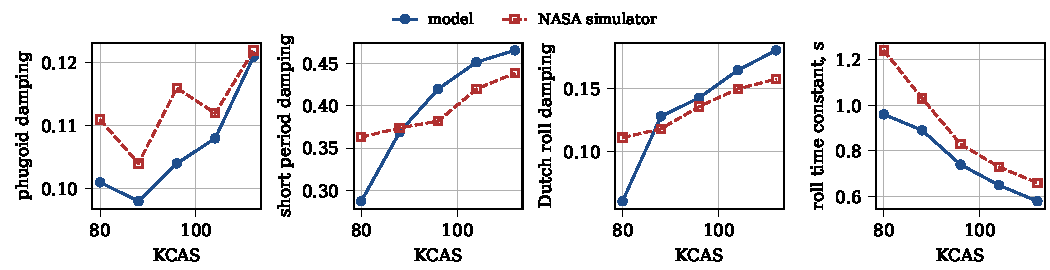
\includegraphics[width=\textwidth]{modes.pdf}
\caption{Mod III's modes against the simulator's \textbf{(S)}.}\label{fig:modes}
\end{figure*}

\subsection{High lift}\label{sec:hl}
\textbf{(C)} With the CFD's thrust, Mod IV at 58\,KCAS and flaps 30 reaches $C_{L\max}=4.53$ (4.40--4.58), the propellers adding 1.23 to 1.63. Figure~\ref{fig:wake} and table~\ref{tab:wake} show the three slipstreams tried. With no constant at all the ring wake halves the plain jet's error and brings moment and drag to their limits. Lift stays about 0.3 high, and one constant takes it inside the solvers' spread, as well as the three it replaced.

\begin{table}[t]
\centering\small
\caption{Slipstream models at 58\,KCAS, flaps 30.}\label{tab:wake}
\begin{tabular}{@{}lrrr@{}}
\toprule
 & Constants & $C_{L\max}$ & $C_L$ error \\
\midrule
Limit & & 4.40--4.58 & 0.078 \\
Jet, as first fitted, discs alternating & 3 & 4.52 & 0.078 \\
Jet, no fit & 0 & 5.55 & 0.690 \\
Ring wake, no fit & 0 & 4.99 & 0.327 \\
Ring wake & 1 & 4.54 & 0.072 \\
\bottomrule
\end{tabular}
\end{table}

\begin{figure}[t]
\centering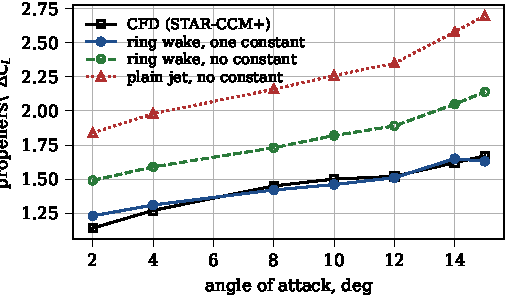
\includegraphics[width=\columnwidth]{slipstream.pdf}
\caption{Lift the high-lift propellers add, with the CFD's thrust \textbf{(C)}.}\label{fig:wake}
\end{figure}

\subsection{A motor lost}\label{sec:upset}
\textbf{(S)} The published failure, no pilot, 6000\,ft, 95\,KCAS \cite{cm}, is described as takeoff flaps and gear down. Its traces can't be that. Its trim incidence of 8.4$^\circ$ and Mod II's 5.4$^\circ$ both sit on the cruise line of the Mod II paper's figures, and its airspeed falls at the rate of about 115\,lbf lost, where takeoff flaps and gear need 180 a motor. The table model, flown clean, lands on every trace at once (fig.~\ref{fig:upset}). This is an inference from the published numbers, not something stated. The test now flies clean, with its targets and limits as they were, and the takeoff-flap run still prints.

\begin{figure*}[t]
\centering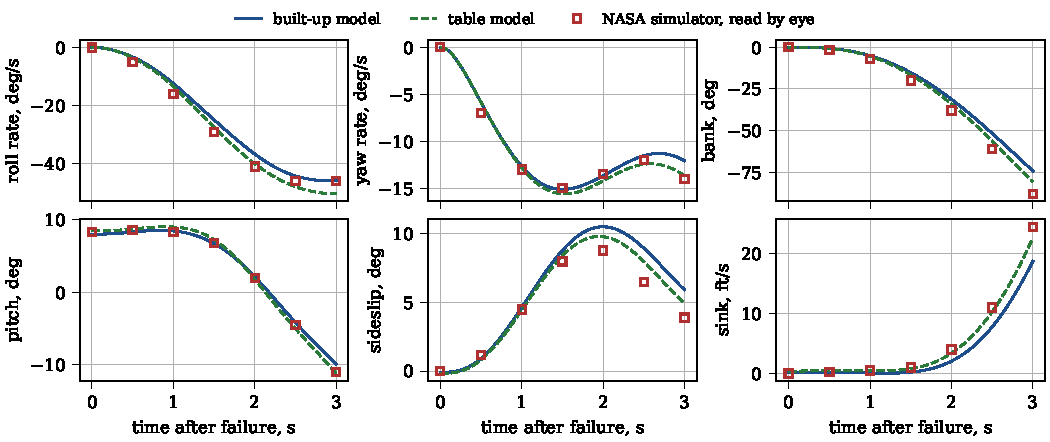
\includegraphics[width=\textwidth]{upset.pdf}
\caption{The left motor lost at 6000\,ft, 95\,KCAS, no pilot, flown clean \textbf{(S)}.}\label{fig:upset}
\end{figure*}

Flown clean, the built-up model at first rolled too little, $-60^\circ$ at 3\,s where the table model gave $-81^\circ$. That was a real departure from the CFD, in two parts: sideslip's roll near stall, and one propeller's own roll. With both fitted it gives bank $-75^\circ$, pitch $-10.1^\circ$, heading $-23.2^\circ$, peak roll rate $-46$\,deg/s and sideslip 10.5$^\circ$, sink 19.1\,ft/s, against about $-87^\circ$, $-11.5^\circ$, $-23^\circ$, $-47$, 9.1$^\circ$, 24.5. The check that first flagged the sideslip as twice the published figure was comparing unlike configurations.

\subsection{Climbs, control and failures}
\textbf{(S)} With a motor out and feathered Mod III sinks 418\,ft/min (450), and 315 (300) with a traction bus out. Minimum control speed is 83.3\,KCAS (85), set by the rudder. Every row of the published failure list \cite{sim3} is present and does what the row says. A contactor failure at 58\,KCAS costs $\Delta C_L$ $-0.30$ and $-0.34$ (read as $-0.30$ and $-0.35$) \textbf{(C)}.

Six climbs miss. Mod III at full power climbs 597\,ft/min (430), and at 2400\,rpm 426 (270); DiTTo at 84\,KIAS 1151 (1000), and with a contactor out 599 and 893 (480 and 740). With both cruise motors running every climb sits 70 to 170\,ft/min above the simulator's; the cruise propellers' drag reduction from the CFD (section~\ref{sec:wake}) added about 80 of that, and 20 to 40 with one out. NASA's database holds the same increments, each side's on $J$ and blade pitch \cite{tm}.
The rest is thrust. Clean, against NASA's performance estimates, made with its simulator's own models \cite{perf}: with no thrust the model's $L/D$ at 8000\,ft is within 3\,\% of NASA's from 120 to 200\,KTAS (14.9 against 14.8 at the peak, 13.6 against 13.3 at 150\,KTAS), with more drag below that, yet at maximum continuous power and 2500\,ft it climbs 785 to 826\,ft/min at 100 to 110\,KTAS against NASA's 600, and 90 to 110 more from 137 to 163\,KTAS. The thrust NASA's figures imply is about 3\,\% under the model's at $J=1.35$ and nearer 18\,\% at 0.9. NASA's cruise propellers carry an installed loss matched to $J$ from Mod I's flight-tested thrust \cite{perf}, not published; this model has the uninstalled tables both start from. That loss isn't fitted: its size isn't known, one that swings from 3 to 18\,\% reads more as compensation than as an installation, and a flat 8\,\% that brings the climbs with both motors inside their limits takes the bus-out ones outside. Nor is it the slipstream counted twice: in the climb the cruise propellers' wake takes off half to two-thirds of the CFD's drag reduction, and with no wake at all the model still climbs 45 to 130\,ft/min over NASA's figure. DiTTo with a motor out gives 86 and 455\,ft/min (360 and 530). The published drop at 97\,KIAS implies 108\,lbf lost from a motor whose published tables give 173, and the table model drops by the same as the built-up one, so this isn't the built-up model's. The arithmetic is short: climb lost is thrust lost times true airspeed over weight, so about 170\,lbf net at 170\,ft/s on 3075\,lb costs some 560\,ft/min before any rudder and aileron drag. The model loses 643, NASA 360. On the real P2006T one engine out costs 81\,\% of the climb \cite{afm}; here it's 90\,\% at 97\,KIAS and 59\,\% at 84, against NASA's 50 and 47. That comparison is loose, since a tip motor is about 30\,\% of the thrust and not half, and NASA's simulator may hold an effect its published tables don't show. DiTTo with a bus out gives $-174$ and 87 ($-100$ and 100).

\textbf{(C)} Ground effect is fitted, so flaps 30 no longer tests anything. Flaps 10's worst points stay at 0.060 and 0.123, and with the propellers on 0.140 and 0.312, speeds averaged.

\subsection{Wing bending}
\textbf{(M)} Fitted to the vibration test's first modes (2.25 and 6.55\,Hz, 2.14 antisymmetric). The nacelle's rotary inertia about the fore-and-aft axis is estimated from its size, not fitted: its 134\,lb as a solid cylinder filling its widest section, 0.93\,kg\,m$^2$. Unfitted: with the tip masses, second bending 17.00\,Hz (15.76) and 15.90 (14.82); clean, second bending 27.78 (26.36) and 25.76 (23.90), and antisymmetric first bending 6.06 (5.76), 5.2\,\% high against a limit of 5, a narrow miss. Without the nacelle's inertia, second bending with the tip masses was 18.50 and 17.06\,Hz, 17 and 15\,\% high, because that mode turns the tip most. The model only flies the first mode. \textbf{(S)} Whole aircraft 2.39\,Hz (2.31) for Mod III and 2.37 (2.29) for Mod IV. In JSBSim with the air nearly gone the modes ring at the beam's frequencies within 1\,\%; in flight they're damped at every speed to $V_{NE}$. There's no torsion, so no flutter prediction. Bending off gives the rigid model's forces exactly.

\subsection{Cockpit and FlightGear}
\textbf{(D)} The avionics buses, sheds and propeller modes pass against the handbook. In FlightGear each overhead and lower switch, the wired breakers, light tests, alerts, manual pitch, the lever's feather stop, the high-lift logic, flaps, Autostart and Autostop were driven by the property each control sets. All 113 clickable controls have their objects and Nasal. Hands off in cruise it holds height within 3\,ft in 60\,s. Real mouse clicks were not automated.

\subsection{Sound}
Every sound plays on one scale, a full-scale sample at volume 1 being 112.5\,dB re 20\,$\mu$Pa, in the cockpit and outside alike. The propellers, motors, the wind on the windscreen and the gear in the airflow are computed by PyWopWop \cite{pww}, the last by Fink's method \cite{anopp} as for the ASK~21's fixed wheels: at 90\,kt the gear is 66.7\,dB(A) at 30\,m, about one cruise propeller's level, and 73.3 in the cockpit, some 16\,dB under the wind. So are the tyres rolling, each wheel on its own speed: scaled from a measured truck tyre, outside they come within 0.5\,dB of the one light aircraft measured (60.5 against 60\,dB(A) at 30\,m), and in the cockpit their level comes from a recorded landing in a P2006T's cabin, set against the wind: three wheels make 86\,dB(A) at 30\,kt and 89.5 at 60, perhaps up to 3\,dB loud. The touchdowns are PyWopWop's too, each wheel's on its own. The flight model turns each wheel: on the runway friction spins it up, the tyre's sliding grip on its strut's force, until it rolls; in the air its brake's pads and its bearings slow it, 3\,N\,m a main wheel and 0.5 the unbraked nose, estimates with no measurement behind them, which stop a main wheel from 85\,kt in some 14\,s, and the pedal stops it at once. As a wheel's weight comes on, the flight model holds its sink rate and its slip, the ground speed less its rim's. The tyre slides until it rolls, losing $I(\mathit{slip}/r)^2/2$ whatever the load, and the strut sets how fast the load comes, its damping slowing the sink while the wing sheds the weight, so a firm touchdown squeals short and a gentle one long, the squeal following the load as the recorded one does; a wheel back on the runway after a hop is still turning, and quiet. The share of that loss heard and its spectrum come from the same P2006T landing, the nose tyre's spectrum from a glider's: at 60\,kt of slip a main wheel's squeal is 83\,dB(A) of sound exposure in the cockpit and 68 at 30\,m, the nose wheel's 79 and 67. Each wheel's files are one waveform under different envelopes, cross-faded by amplitude over the slip and the sink rate, so a touchdown between them is one event at the law's level, within 0.2\,dB, the energy their differences cost put back. The strut's thump, the force its damping puts into the airframe, was at the edge of hearing in that recording, so its estimate is uncertain; it plays at it, a main wheel's from 69\,dB(A) at 0.25\,ft/s to 81 at 1\,ft/s, a firmer one through a soft knee where it would pass full scale, 3\,dB under its estimate at 2\,ft/s and 7 at 4. Those two recordings are the only ones used. Mods III and IV were never heard, so the rest is computed, not checked; the motors' levels and the wind's 91\,dB(A) at 110\,kt are the least certain. The gear's pump and locks and the flap motor use stock samples at stated levels, all estimates: none has a measurement behind it on this aircraft. The aural alert is set 15\,dB over the cockpit's noise at 100\,kt, after ISO~7731. A check reads each level back from the sound file, and refuses any condition FlightGear wouldn't load: one did, silencing the tyres until a recorded landing showed it.

\section{Corrections found during validation}\label{sec:review}
\begin{itemize}
\item A blade-element solver took the first root it met, and lightly loaded sections have false ones. Phugoid damping, which hangs on how thrust moves with speed, exposed it.
\item The rudder scale sat ahead of a table ending at 26$^\circ$, stopping it at 17$^\circ$. Later the fin's table itself proved a quarter weak at full travel.
\item A wing's divide by a speed near zero, and JSBSim's $b/2V$, threw the aircraft into NaN at rest with the rotors turning. Both are floored at 30\,ft/s.
\item Reading JSBSim's accelerations for the panels' coupling gave wrong frequencies and negative damping; it's solved in the system now. Raw roll rate fed to the ailerons pumps the 3.55\,Hz mode up, so a test pilot's rate passes a 0.25\,s lag.
\item The force graph couldn't start in FlightGear until it became a system channel.
\item FlightGear's default electrical system was running beside the model's and overwriting one voltage. It's off.
\item The door handles called a module the package didn't load.
\item The high-lift propellers first alternated along each wing, from a loose reading of the simulator paper. Turned as the geometry and the CFD have them, maximum lift rose by 0.06 with no constant changed, a contactor failure's yaw came inside its limit, which had been a miss, and the propellers' sound outside moved by up to 10\,dB, because the side view hears the rising blades.
\item The cruise blades in the visual model were pitched for the opposite rotation to their animation.
\item The failure test ran the wrong configuration (section~\ref{sec:upset}), and minimum control speed was read from an unsolved point.
\item The gear retracted on the ground. The flight manual shows only a knob to pull first, and other sources differ on a squat switch. A guard was added as a simulator choice.
\item The parked check asked for wings level, though the published CG sits 1.19\,in left of the centre line \cite{sim3}. The mains' springs and the CG's height give $-0.17^\circ$ for that, which the model shows; the check now asks for the statics' lean, within the same $0.1^\circ$.
\item The brakes stopped the P2006T at the tyre's grip, 0.7\,g, in 138\,m against the manual's 209. The manual's table is for grass and paved is only 2\,\% shorter, so its brakes, not the tyres, set the stop. Given a force fitted to the paved roll, the same landing on grass, at the published grip of a tyre there \cite{gd}, stops in 208\,m against the manual's 213, an unfitted test. The X-57's brakes now hold it to half lever at 2700\,rpm, and its takeoff test starts rolling, as the published technique does \cite{dt}.
\item The discs took the air at the centre of gravity, so the airplane's turning changed neither their thrust nor their in-plane force. Each now takes its own: the wingtip discs add 18\,\% to the yaw damping, and Mod IV's fixed-mode check, which passed, now misses the simulator's Dutch roll damping, by 0.085 against 0.05 with the sideslip fit below.
\item With the high lift on, the power-off fit for sideslip's roll and yaw was switched off whole, on the ground that blown sections don't stall. At 2$^\circ$, far from stall, it still holds the high sideslip's yaw, +0.013 at 20$^\circ$, flaps 30, which the CFD with the propellers on shows too. That part now stays: power-on yaw from sideslip went from 16 to 8\,\% rms, roll from 26 to 23, inside the limit.
\item The rates' correction stayed whole with the high lift running, and near stall it stood for unblown sections stalling, so blown roll damping was counted twice: $-1.19$ at 12$^\circ$, flaps 30, 58\,KCAS, where the strips alone and the CFD's forced oscillation with the propellers on both give $-0.84$. Held below stall, the model comes to the powered forced-oscillation CFD within 0.074 rms in $C_{l_p}$, from 0.222, and 0.024 in $C_{n_p}$, from 0.061. Those runs were flown at a fifth of the power-off runs' frequency, so comparing the two, as the CFD's own report does, mixes frequency with power; at one frequency, thrust adds no yaw damping to the airframe in either the CFD or the model, and roll damping in the model grows half as fast as in the CFD.
\item The strip over the cabin sat inside the fuselage's circle, where the doublet doesn't hold, and its clamp left it 14\,\% of a wing's response to incidence: the loading dipped at the roots and the fits made it up outboard. It now carries the carry-through lift as wing. After the refit, ground effect with the propellers on came inside its limit (0.138 against 0.15) and flaps 20, unfitted, closed from 0.026 to 0.017 in $C_m$.
\item The cruise propellers' swirl was spread evenly across the jet and turned only the strips' incidence, not their force. Against the power-on CFD, one propeller running as it does there, drag rose with thrust where the CFD's falls, and lift, pitch and the strips' own roll came to 0.73, 0.39 and 0.71 of the CFD's. Given the Goldstein loading NASA's CFD gives them, and the force turned with the swirl, they come to 1.07, 0.88 and 1.03, and drag to 1.01, nothing fitted (section~\ref{sec:wake}). The climbs rose about 80\,ft/min with both cruise motors running, 20 to 40 with one out or a bus lost: three DiTTo climbs that passed now miss, two that missed pass. A comparison before that ran both propellers against the CFD's one, and read the lift as twice the CFD's.
\item The wing beam carried the nacelle as a point mass. Given the nacelle's rotary inertia, estimated from its size, second bending with the tip masses came within 8\,\% of the vibration test, from 17\,\% high. The clean wing's antisymmetric first bending moved from 5.0 to 5.2\,\% high and now misses its 5\,\% limit.
\end{itemize}

\section{Assessment}\label{sec:assess}
\Nmiss{} checks miss. They fall into four kinds:
\begin{itemize}
\item \textbf{A source's figure in doubt.} The P2006T flight paper's short period and lift and moment slopes. That aircraft flies, so the reasons given can be weighed against other flight data.
\item \textbf{Sources that can't all be met.} The climbs with both cruise motors running, 70 to 170\,ft/min above the simulator's, whose cruise propellers carry an unpublished installed loss this model doesn't; the DiTTo motor-out climbs against the published motor tables, a mismatch inside the published figures that no flight can settle; the Mod II simulator's Dutch roll and phugoid against the flight test.
\item \textbf{Limits written for another model.} Several mode limits written for the table model.
\item \textbf{Real or open.} Ground effect at flaps 10 and with the propellers on; a 12\,\% high lift slope on the P2006T; the aileron's pitching moment; the clean wing's antisymmetric first bending, 5.2\,\% high against 5; $C_{Y\beta}$; the Mod II simulator's roll time constant.
\end{itemize}
The motors' and rotors' inertias, loads, the torque rate and the speed-loop gains are estimates. Not modelled: torsion and flutter, the slipstreams' width changing with thrust and their path over the wing with incidence, dynamic inflow, the motors' temperatures. Mods III and IV never flew, so a pass against CFD or a simulator shows agreement with a prediction and no more, and a miss doesn't show which of the two is wrong. This work isn't connected with or endorsed by NASA, Tecnam or the aircraft's makers.

\section{Conclusions}\label{sec:concl}
\begin{itemize}
\item A built-up model of the X-57 Mods III and IV, each of its fourteen propellers a disc with its own speed, its wing strips in their own slipstreams and its wing bending, runs in plain JSBSim at 120\,Hz, generated from published data.
\item Proved on the P2006T it passes the flight manual, and a second source shows the flight test's short period to be a method artefact.
\item A ring-vortex slipstream with one constant does as well as a jet with three, and with none it halves the error of a plain jet.
\item The published motor failure is reproduced in time history, once flown in the clean configuration its own traces show.
\item Limits were set first and never moved; one target was corrected for the published CG. \Npass{} checks pass and \Nmiss{} miss, each with its cause or marked open.
\end{itemize}

\begin{thebibliography}{99}\small
\bibitem{tm} M.\,A.\ Frederick, M.\,S.\ Smith, S.\,Y.\ Yoo, R.\ Wallace, J.\,C.\ Duensing, J.\,A.\ Housman, K.\,A.\ Deere, J.\,K.\ Viken et al., \emph{Development of the X-57 Aerodynamic Database}, NASA/TM-20250001715, 2025.
\bibitem{hlp} N.\,K.\ Borer and M.\,D.\ Patterson, \emph{X-57 High-Lift Propeller Control Schedule Development}, NTRS 20205010303.
\bibitem{gvt} S.\ Truong, K.\ Bhamidipati, S.-F.\ Lung, N.\ Spivey, R.\ Truax and J.\ Winkel, \emph{X-57 Mod III Wing Ground Vibration Test}, NTRS 20240011864.
\bibitem{tun} B.\,L.\ Litherland, N.\,K.\ Borer and N.\,S.\ Zawodny, \emph{X-57 ``Maxwell'' High-Lift Propeller Testing and Model Development}, NTRS 20210016834.
\bibitem{tun2} B.\ Litherland and N.\ Borer, \emph{X-57 ``Maxwell'' High-Lift Propeller Test for Improved Thrust Measurements and Slipstream Velocities}, AIAA Aviation Forum, 2022, NTRS 20220006506.
\bibitem{icd} NASA, \emph{X-57 Cockpit Interface Control Document}, ICD-CEPT-006 rev.~E, NTRS 20230016539.
\bibitem{pc} K.\,M.\ McLaughlin, R.\,N.\ Vidyasagar, J.\ Lucht, A.\ Waddell, J.\ Rudy and A.\,F.\ Curry, \emph{X-57 Flight Systems Integration Path}, NTRS 20240005892.
\bibitem{tr} S.\ Clarke, J.\ Terry, K.\ Harris and D.\ Avanesian, \emph{X-57 Traction Power and Command Systems Development}, NTRS 20240009560.
\bibitem{pc17} S.\ Clarke, M.\ Redifer, K.\ Papathakis and A.\ Samuel, \emph{X-57 Power and Command System Design}, NTRS 20170005797.
\bibitem{sim3} R.\ Wallace, J.\ Reynolds, D.\ McMinn and D.\ Cox, \emph{Development of the X-57 Mod III/IV Piloted Simulator and Discussion of the Resultant Flying Qualities Predictions}, NTRS 20240006496.
\bibitem{sim2} R.\ Wallace, J.\ Reynolds, M.\ Frederick, D.\ McMinn, D.\ Cox and N.\ Borer, \emph{Development of the Mod II X-57 Piloted Simulator and Flying Qualities Predictions}, NTRS 20230004174.
\bibitem{cm} R.\ Wallace, J.\ Reynolds and N.\ Borer, \emph{Mitigation of High Lateral Asymmetry Rates Due to Loss of a Cruise Motor on the X-57 Mod III Aircraft}, NTRS 20240006682.
\bibitem{dt} N.\,K.\ Borer, R.\,D.\ Wallace, J.\,R.\ Reynolds, D.\,E.\ Cox, C.\ Sales, T.\,L.\ Williams and W.\,M.\ Ringelberg, \emph{Distributed Thrust Takeoff for the NASA X-57 Mod IV Flight Demonstrator}, NTRS 20240010539.
\bibitem{fl} K.\,K.\ Bhamidipati, C.\ Pak, R.\ Truax, J.\,P.\ Winkel, S.\ Rosario, S.\,E.\ Cutright, S.\,J.\ Massey and C.\,D.\ Wieseman, \emph{Classical Flutter Analysis of X-57 Aircraft Mod II, III, and IV Configurations}, NTRS 20240007439.
\bibitem{hlm} D.\,L.\ Hall, J.\,C.\ Chin, A.\,D.\ Anderson, J.\,T.\ Thompson, A.\,D.\ Smith and K.\,P.\ Duffy, \emph{Development of a Maxwell X-57 High Lift Motor Reference Design}, NTRS 20190029267.
\bibitem{chin} J.\,C.\ Chin, S.\,L.\ Schnulo, T.\,B.\ Miller, K.\ Prokopius and J.\ Gray, \emph{Battery Performance Modeling on Maxwell X-57}, 2019.
\bibitem{gd} L.\,J.\ Newton and R.\,D.\ Wallace, \emph{X-57 Ground Dynamics Modeling and Analysis}, NTRS 20220005440.
\bibitem{afm} Tecnam, \emph{P2006T Aircraft Flight Manual}, Doc.\ No.\ 2006/044.
\bibitem{nic} F.\ Nicolosi, A.\ De Marco and P.\ Della Vecchia, \emph{Stability, Flying Qualities and Parameter Estimation of a Twin-Engine CS-23/FAR 23 Certified Light Aircraft}, AIAA 2010-7947.
\bibitem{perf} N.\,K.\ Borer, \emph{Flight Performance Estimates for the NASA X-57 Distributed Electric Propulsion Flight Demonstrator}, NTRS 20240010807, 2024.
\bibitem{gold} S.\ Goldstein, \emph{On the Vortex Theory of Screw Propellers}, Proc.\ R.\ Soc.\ Lond.\ A 123, 440--465, 1929.
\bibitem{hk} H.\,H.\ Heyson and S.\ Katzoff, \emph{Induced Velocities Near a Lifting Rotor with Nonuniform Disk Loading}, NACA Report 1319, 1957.
\bibitem{dv} K.\,A.\ Deere, J.\,K.\ Viken, M.\,R.\ Wiese and N.\,L.\ Farr, \emph{Computational Analysis of the X-57 Maxwell Airplane, the Landing Configuration with High-Lift Blowing and Aileron Deflections (Preliminary Fuselage)}, NASA/TM-20230010662.
\bibitem{deere} K.\,A.\ Deere, S.\,A.\ Viken, M.\,B.\ Carter, J.\,K.\ Viken, M.\,R.\ Wiese and N.\ Farr, \emph{Computational Analysis of Powered Lift Augmentation for the LEAPTech Distributed Electric Propulsion Wing}, AIAA Aviation Forum, 2017, NTRS 20170005861.
\bibitem{borer} N.\,K.\ Borer, M.\,D.\ Patterson, J.\,K.\ Viken, M.\,D.\ Moore et al., \emph{Design and Performance of the NASA SCEPTOR Distributed Electric Propulsion Flight Demonstrator}, NTRS 20160010157.
\bibitem{anopp} W.\,E.\ Zorumski, \emph{Aircraft Noise Prediction Program Theoretical Manual}, NASA TM-83199, 1982.
\bibitem{pww} \emph{Rotorcraft and Glider Sound for Flight Simulators from First Principles} (PyWopWop), technical report, 2026.
\end{thebibliography}
\end{document}
